%% Adaptado a partir de :
%%    abtex2-modelo-trabalho-academico.tex, v-1.9.2 laurocesar
%% para ser um modelo para os trabalhos no IFSP-SPO

\documentclass[
    % -- opções da classe memoir --
    12pt,               % tamanho da fonte
    openright,          % capítulos começam em pág ímpar (insere página vazia caso preciso)
    %twoside,            % para impressão em verso e anverso. Oposto a oneside
    oneside,
    a4paper,            % tamanho do papel. 
    % -- opções da classe abntex2 --schwinn
    % Opções que não devem ser utilizadas na versão final do documento
    %draft,              % para compilar mais rápido, remover na versão final
    paginasA3,  % indica que vai utilizar paginas em A3 
    MODELO,             % indica que é um documento modelo então precisa dos geradores de texto
    TODO,               % indica que deve apresentar lista de pendencias 
    % -- opções do pacote babel --
    english,            % idioma adicional para hifenização
    brazil              % o último idioma é o principal do documento
    ]{ifsp-spo-inf-ctds} % ajustar de acordo com o modelo desejado para o curso

% ---
% Pacotes básicos 
% ---
%\usepackage[utf8]{inputenc}     % Codificacao do documento (conversão automática dos acentos)
% ---

%\usepackage{style}
        

% --- 
% CONFIGURAÇÕES DE PACOTES ADICIONAIS UTEIS
% --- 


% ---
% Informações de dados para CAPA e FOLHA DE ROSTO
% ---
\titulo{Análise dos Processos e Mecanismos de Contratação - EY}


\renewcommand{\imprimirautor}{
\begin{tabular}{lr}
Any Gabrielly Gomes dos Santos & SP3050122 \\
John Henrique Mendonça Souza & SP3039072 \\
Jorge Wilson Silva Jardim & SP3056406 \\
Lucas de Macedo Polezel & SP305411X \\
\end{tabular}
}

\disciplina{RHUA1 - Recursos Humanos em Tecnologia da Informação}


\data{27 de Setembro de 2020}

\renewcommand{\orientadorname}{Professor:}
\orientador{Luis Fernando Aires Branco Menegueti}


% ---


% informações do PDF
\makeatletter
\hypersetup{
        %pagebackref=true,
        pdftitle={\@title}, 
        pdfauthor={\@author},
        pdfsubject={\imprimirpreambulo},
        pdfcreator={LaTeX with abnTeX2 using IFSP model},
        pdfkeywords={abnt}{latex}{abntex}{abntex2}{IFSP}{\ifspprefixo}{trabalho acadêmico}, 
        colorlinks=true,            % false: boxed links; true: colored links
        linkcolor=blue,             % color of internal links
        citecolor=blue,             % color of links to bibliography
        filecolor=magenta,              % color of file links
        urlcolor=blue,
        bookmarksdepth=4
}
\makeatother
% --- 


% ----
% Início do documento
% ----


\begin{document}


\frenchspacing 




% -- lista de pendencias gerada pelo todonotes
% -- altere opções do usepackage para remover na versão final....

\newpage

% ----------------------------------------------------------
% ELEMENTOS PRÉ-TEXTUAIS
% ----------------------------------------------------------
\pretextual

% ---
% Capa
% ---
\imprimircapa


% ---

% ---
% Folha de rosto
% (o * indica que haverá a ficha bibliográfica)
% ---
\imprimirfolhaderosto
%\imprimirfolhaderosto*
% ---


% -- resumo obrigatório
% ---
% RESUMOS
% ---

% resumo em português
\setlength{\absparsep}{18pt} % ajusta o espaçamento dos parágrafos do resumo
\begin{resumo}

 Essa proposta de trabalho é referente a primeira etapa de um projeto da matéria de Recursos Humanos em Tecnologia da Informação. Nesse estudo foram analisados processos e mecanismos de contratação da empresa Ernst & Young Global Limited, dividido em três partes, as quais se debruçam sobre, a empresa de um modo geral, o recrutamento e uma crítica sobre o processo seletivo, respectivamente. O intuito desse projeto é de identificar, analisar e debater, ferramentas e técnicas utilizadas na contratação, de forma a fomentar um senso crítico fundamentado na teoria, a qual pudemos ter em sala de aula.


 \textbf{Palavras-chaves}: recursos humanos. projeto. estudo.
\end{resumo}

% resumo em inglês
\begin{resumo}[Abstract]
 \begin{otherlanguage*}{english}
This work proposal is related to the first stage of a Human Resources in Information Technology project. In this study, the hiring processes and mechanisms of the company Ernst & Young Global Limited were analyzed, divided into three stages, which focus on, the company, the recruitment process and a criticism about it, respectively. The purpose of this project is to identify, analyze and debate, tools and techniques used in recruitment process, in order to stimulate a critical sense based on theory, which we were able to have in the classroom.


   \vspace{\onelineskip}
 
   \noindent 
   \textbf{Key-words}: human resources. project. study.
 \end{otherlanguage*}
\end{resumo}



% ---
% inserir o sumario
% ---
\pdfbookmark[0]{\contentsname}{toc}
\tableofcontents*
\cleardoublepage
% ---


% ----------------------------------------------------------
% ELEMENTOS TEXTUAIS
% ----------------------------------------------------------
\textual


% ----------------------------------------------------------
% Introdução (exemplo de capítulo sem numeração, mas presente no Sumário)
% ----------------------------------------------------------
\chapter[Introdução]{Introdução à EY}

\section{Apresentação da empresa}
A EY, também conhecida como Ernst & Young Global Limited, é uma empresa multinacional de serviços profissionais ligados a área contábil, sendo considerada junto com a Deloitte, KPMG e PricewaterhouseCoopers uma das maiores empresas do mundo dentro desse ramo. 
Em 2019, a EY se destacou como a sétima maior organização privada dos Estados Unidos, e, além disso, tem sido continuamente classificada na lista das 100 melhores empresas para se trabalhar da revista Fortune nos últimos 21 anos, mais do que qualquer outra empresa de contabilidade.


\section{Histórico da empresa}
A EY é uma empresa que nasceu da fusão em 1989 de duas empresas britânicas de contabilidade, sendo elas a Ernst & Whinney e Arthur Young & Co. Desde 2013 a empresa passou a se chamar EY e mudou seu slogan para \textit{Building a Better Working World}. Hoje possuí mais de 700 escritórios que estão espalhados em mais de 150 países com 260 mil funcionários; No Brasil são 14 escritórios em 12 cidades com 5 mil funcionários. 
Atualmente a EY possui quatro linhas de serviços principais: Consultoria, Auditoria, Impostos e Transações. Com esses pilares eles buscam ajudar organizações privadas ou publicas a capitalizarem mais oportunidades, independente da estrutura das empresas que a contratam.


\section{Missão}
"Na EY, nosso propósito é construir um mundo de negócios melhor. Os \textit{insights} e serviços de qualidade que oferecemos ajudam a construir confiança nos mercados de capitais e nas economias de todo o mundo. Desenvolvemos líderes excepcionais que se unem para cumprir nossas promessas a todos os nossos acionistas. Ao fazê-lo, desempenhamos um papel fundamental na construção de um mundo de negócios melhor para as nossas pessoas, os nossos clientes e as nossas comunidades."

\fonte{Disponível em: <https://www.ey.com/pt_br/who-we-are/>. Acessado em: 23 de Setembro de 2020}

\section{Visão}
"Na EY, fazemos todo o possível para tornar o mundo melhor. É o que afirma nossa afirmação "Construindo um mundo de trabalho melhor". Com nosso conhecimento abrangente e a qualidade de nossos serviços, fortalecemos a confiança nos mercados de capitais e economias em todo o mundo. Dessa forma, contribuímos de maneira importante para mudar o mundo - para nossos funcionários, clientes e sociedade como um todo."

\fonte{Disponível em: <https://www.ey.com/pt_br/nossa-lideranca>. Acessado em: 23 de Setembro de 2020}

\section{Valores}
"Na EY, nossos valores nos definem e são o alicerce da nossa cultura. Integridade, respeito e espírito de equipe estão no nosso DNA. Agimos com energia, entusiasmo e coragem para liderar. Tudo isso para construir relacionamentos baseados em fazer a coisa certa.

A EY é a empresa mais globalizada em pensamento, estrutura, processos e oportunidades.

Na EY, somos uma equipe de alta performance. Nosso sucesso está no desenvolvimento de nossas pessoas. Por isso, focamos no enorme potencial que cada pessoa traz para o grupo. Vivenciamos diariamente nossos valores com inclusão total da diversidade, forte investimento em educação e liderança transformadora."

\fonte{Disponível em: <https://beyellow.com.br/sobre-a-ey/>. Acessado em: 23 de Setembro de 2020}




% Para facilitar a manutenção é sempre melhore criar um arquivo por capitulo, para exemplo isso não é necessário 
% Para facilitar a manutenção é sempre melhore criar um arquivo por capitulo, para exemplo isso não é necessário 

%---------------------------------------------------------------------------------------
\chapter{Etapas de Processo Seletivo}

O processo seletivo da Ernst & Young é dividido em seis etapas, as quais se estendem por um período de dez meses, sendo os dois primeiros meses apenas para inscrições, e, a partir do terceiro mês o processo avança para as etapas subsequentes, porém as inscrições permanecem até o último mês do processo.


\begin{figure}[h]
	\centering
	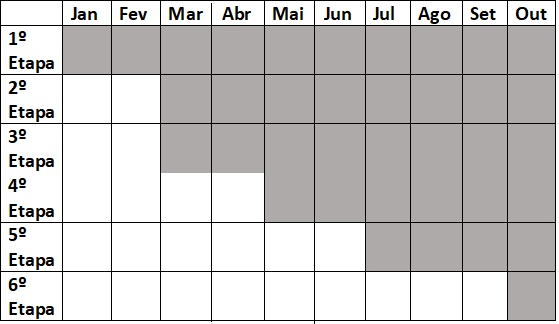
\includegraphics[scale=0.8]{processo.jpeg}
	\caption{Tempo total investido em cada etapa do processo seletivo}
	\label{fig:mesh1}
	
\end{figure}


\section{Inscrição e Avaliação Curricular}{

A avaliação curricular é uma etapa online que consiste em acessar o site do programa de \textit{Trainees} e realizar a inscrição, o que já direciona o candidato a vaga que mais adequada ao perfil do mesmo, e, além dessa maneira, as vagas ficas disponíveis em outras plataformas direcionadas ao recrutamento online, onde são amplamente divulgadas.
Na plataforma de recrutamento o processo seletivo fica mais acessível, pois, além de realizar cruzamento dos dados dos currículos como os pré-requisitos das vagas, onde sugere para os usuários vagas de acordo com o perfil do mesmo, também dá suporte durante o andamento de todas as etapas. 
Essa etapa garante uma maior agilidade e eficiência na análise de currículos de candidatos, além de tornar o processo mais visível por estar em uma plataforma na qual os usuários estão estritamente ligados para buscar uma vaga de emprego, onde a plataforma sugere para usuários a vaga com maior aderência.
As redes sociais também são amplamente utilizadas para divulgação do programa de \textit{Trainees} da EY, onde seus próprios colaboradores realizam postagens sobre o programa incentivando aos interessados a se inscreverem na oportunidade.
Nessa etapa os candidatos são analisados e selecionados com base nos requisitos mínimos preestabelecidos com base em sua formação e habilidades específicas (neste caso o Inglês).


\begin{table}[htb]
\centering
\caption{Pré-requisitos}
\label{tab-exemplo}
\begin{tabular}{p{2.8cm}|r|r|r|r}
    \hline
   \textbf{Curso} & \textbf{Formação}  & \textbf{Nível de Inglês} \\
    \hline
    Ciências Contábeis & Janeiro de 2017 a dezembro de 2022 & Básico  \\
    \hline
    Cursos de T.I. & Janeiro de 2017 a dezembro de 2021  & Básico \\
    \hline
    Administração de Empresas, Ciências Atuariais, Economia, Relações Internacionais, Comércio Exterior, Direito, Engenharia (todas), Estatística, Física, Matemática, Psicologia, Marketing, Publicidade e Propaganda, Design & Janeiro de 2017 a dezembro de 2021  & Intermediário \\
    \hline
\end{tabular}
\fonte{Disponível em: <https://beyellow.com.br/programa/>. Acessado em: 23 de Setembro de 2020}
\end{table}}



\newpage


\section{Apresentação Institucional e Redação}

A etapa de apresentação é presencial, realizada na Universidade Corporativa da EY, onde cerca de 50 candidatos que foram classificados na etapa dos testes online, são direcionados para uma palestra de apresentação da empresa, suas diversas áreas com vagas disponíveis, o programa de \textit{Trainees} e seus benefícios. Os candidatos ainda podem tirar dúvidas sobre o processo seletivo e a empresa.
Após a apresentação, o candidato recebe uma folha para fazer uma redação, referente a um tema específico, ligado diretamente à proposta e visão da empresa, que é fazer um mundo de negócios melhor. Com quantidade mínima e máxima de palavras, com um intervalo de tempo de 1 hora. 
Essa etapa da ao candidato a possibilidade de especificar a área da empresa na qual deseja atuar, podendo escolher uma ordem de prioridade entre 3 áreas. Sendo assim, o candidato aprovado será direcionado entre as vagas das áreas priorizadas por ele.
Nessa etapa é analisada a capacidade de comunicação escrita dos candidatos, além da capacidade da abordagem correta do tema e a área de atuação escolhida, em relação as vagas disponíveis.




\section{Testes Online e Escolha da Área de Interesse}

Após a avaliação dos pré-requisitos, a redação e escolha da área de atuação, essa etapa consiste em testes online de Português, Lógica, Inglês em caráter eliminatório e Contabilidade Básica em caráter classificatório, esse último sendo apenas para os cursos de Ciências Contábeis, Administração de Empresas e Ciências Atuariais.
Essa etapa consiste em teste de múltipla escolha, com questões que evoluem de básicas a avançadas de cada assunto, para que o candidato seja avaliado e de acordo com a pontuação, mínima de 70\% em cada teste.
Durante essa etapa são avaliados de maneira eliminatória e classificatória conhecimentos gerais necessários, como Português, Lógica e Inglês, e específicos, no caso de Contabilidade Básica.



\newpage

\section{Dinâmica de Grupo}

A etapa de dinâmica de grupo é presencial com 10 candidatos que, inicialmente, são submetidos a um teste, onde devem desenhar uma casa, árvore e uma pessoa, conhecido como teste de personalidade HTP.
Esse teste tem como objetivo mostrar quais são os conflitos escondidos e comuns dentro de cada candidato, além disso o entrevistador pede para que os candidatos se apresentem e solicita que respondam algumas perguntas como: porque quer trabalhar na EY, o que espera do processo, qual é a maior área de interesse de atuação de acordo com o curso, além de explicar o porquê desenhou os elementos solicitados como desenhou.
Após a primeira fase das dinâmicas os candidatos são divididos em dois grupos com cinco participantes cada, onde é apresentado aos grupos um \textit{case} relacionado com a área de atuação na qual os candidatos foram selecionados. Vale evidenciar, que os grupos são mistos, incluindo candidatos dos vários ramos das vagas disponíveis.
Com isso, o grupo tem um tempo limite de dez minutos para desenvolver o \textit{case}, e organizar uma apresentação, com apoio de uma cartolina, com o desenho da solução e desenvolver um \textit{pitch} de três a cinco minutos,onde os grupos são concorrentes e ambos devem tentar convencer o entrevistador a comprar sua solução proposta. Nessa fase da dinâmica, os candidatos serão pressionados pelo entrevistador durante a apresentação, visando colocá-los em um cenário de extrema pressão e desconforto, e, após a conclusão da apresentação, o outro grupo também pode realizar perguntas.
Após o término das apresentações, o entrevistador dá um \textit{feedback} para os grupos, dizendo os pontos fracos e fortes desenvolvidos durante o \textit{case} e expõe que o objetivo da etapa é uma experimentação para saber como cada candidato se sai sob pressão.
Ao final, abre para perguntas e dúvidas relacionadas a empresa e ao processo seletivo.
Durante essa etapa são avaliador quesitos de personalidade dos candidatos, capacidade de desenvolver uma história, liderança, capacidade de trabalho em equipe, capacidade de trabalho sob pressão, capacidade de comunicação verbal e visão ampla de negócios.




\section{Entrevistas Finais}
Essa etapa é subdividida em duas entrevistas de cerca de 30 minutos cada, onde é realizada uma conversa entre o candidato e o Gerente Técnico, e o candidato e um Sócio da EY.


Durante a entrevista com o gerente são feitas perguntas referentes a formação, áreas de interesse e áreas de atuação. Ainda é feito um \textit{case}, onde é avaliada a tomada de decisão do candidato.
Ao final, a entrevista se abre para perguntas, estipulando um limite máximo de perguntas, onde são avaliadas as perguntas feitas pelo candidato, visto que se espera perguntas que consigam extrair boas informações referente aos negócios e carreira.
Durante a primeira entrevista são avaliados conhecimentos técnicos, tomada de decisão, formulação de perguntas e extração de informações.
    
Durante a entrevista com o sócio são feitas algumas perguntas referentes aos objetivos profissionais e áreas de atuação. Novamente é feito um \textit{case}, onde é dada uma situação hipotética ao candidato e é solicitada uma solução objetiva para o caso, com tempo de cinco minutos. Além disso, é dado papel e caneta para que o candidato possa rascunhar sua solução, visto que envolve cálculos. Após dar a solução, é necessário explicar o raciocínio seguido.
Ao final, a entrevista se abre para perguntas, estipulando um limite máximo de perguntas, novamente avaliando as perguntas feitas pelo candidato.
Durante a segunda entrevista são avaliadas a linha de raciocínio do candidato, capacidade de formulação de perguntas e extração de informações.

Ao final, os dois, juntamente com o entrevistador da dinâmica em grupo, fazem uma reunião, onde classificam todos os candidatos entrevistados, definindo os pontos fortes e fracos dos candidatos, além de definir qual será a área inicial de cada candidato.
Vale ressaltar, que essa entrevista é dinâmica, visto que cada entrevistador e cada candidato tem perfil próprio, o ponto em comum entre todas são os pontos de avaliação que os entrevistadores devem extrair com a conversa.


\section{Processo Admissional}
Ao fim de todos os processos a empresa entra em contato com os candidatos, dando o \textit{feedback} positivo ou negativo e informando o motivo dos mesmos. Em casos positivos, é feita a proposta para o candidato. Após a aceitação, o mesmo é instruído a enviar os dados para admissão, e, posteriormente, para realizar o exame admissional. Depois disso, o novo colaborador é apresentado aos termos do contrato, assina a documentação e inicia sua atuação na empresa.





\chapter[Crítica]{Análise crítica dos mecanismos de contratação}

\section{Primeira Etapa}

A etapa de inscrição e avaliação curricular online é muito importante para o processo seletivo da EY, pois através da divulgação feita por meio de plataformas de seleção de candidatos, as vagas são direcionadas e tornam-se mais acessíveis aos possíveis candidatos, economizando tempo dos colaboradores e recursos para realizar a seleção de perfis que se adéquam aos requisitos desejados. Também é viável para o candidato interessado na vaga, pois toda a plataforma fornece o suporte necessário durante essa etapa, dando sugestões de vagas de acordo com o currículo da pessoa. A divulgação do programa de \textit{Trainees} apenas por meio das redes sociais faz com que um público muito grande tenha maior conhecimento da empresa, mas nem todos os interessados são compatíveis com a vaga, tornando um processo de filtragem muito mais lento e assim tomando tempo dos próprios colaboradores que realizam o contato com os indivíduos.
A avaliação curricular e inscrição online dos candidatos mostra-se bem completa, apesar de que nas redes sociais atrai um grande número de pessoas, muitas vezes não-compatíveis. Durante essa etapa há uma filtragem das vagas através da plataforma, fazendo com que as próximas etapas sejam mais objetivas e não consumam tanto tempo e recursos da empresa. 


\section{Segunda Etapa}
A parte da apresentação institucional da empresa EY é fundamental para o processo seletivo, pois é de suma importância que o candidato conheça melhor a empresa e esteja alinhado com os interesses da mesma como a missão, visão e valores. Neste momento o indivíduo perceberá se suas necessidades serão supridas com o trabalho a ser realizado dentro organização, visto que as necessidades do mesmo nem sempre serão atendidas somente pelo dinheiro, mas também por outros fatores. O conhecimento sobre a organização será refletido na motivação do futuro funcionário, já que o mesmo terá conhecimento do trabalho esperado e como ele vai realizar de uma forma que os resultados sejam favoráveis para si, tanto quanto, para a organização posteriormente durante a construção de sua carreira.
Quanto a redação presencial, a mesma mostra-se muito útil na filtragem de dados do candidato, suas áreas de interesse, conhecimento de escrita e de entendimento a fazer algo que foi apresentado, visto que o tema é delimitado e tem que ser seguido, porém, a redação presencial demanda muito tempo e recursos para ser realizada, visto que nesta etapa do processo seletivo há muitos candidatos, cerca de cinquenta pessoas, em média. Sendo assim seria mais viável para a organização antecipar a etapa de testes online a fim de eliminar os candidatos que não cumprem com o ideal desejado pela vaga, dessa maneira reduzindo o número de candidatos durante essa etapa e assim economizando bastante tempo de todos os colaboradores responsáveis pelo processo.

\section{Terceira Etapa}
Essa etapa é uma das etapas mais simples e eficazes de todo o processo de forma geral, pois analisa todos os candidatos que não preenchem os requisitos mínimos desejados para fazer parte do programa através dos testes de conhecimentos aplicados. Apesar de sua simplicidade e sua eficácia, essa etapa poderia ser antecipada no projeto e até mesmo fazer parte da inscrição do candiado, visto que é uma etapa online de classificação e eliminação de candidatos. Caso fosse executada antes da fase de apresentação da empresa da empresa, que é presencial, economizaria muitos recursos investidos pela empresa para a estrutura da apresentação, visto que alguns candidatos que passariam por essa fase já seriam excluídos do processo. 

\section{Quarta Etapa}
Nessa etapa do processo seletivo da EY não há muitas considerações a serem feitas, pois pelas descrições e experiência de um dos integrantes do grupo o processo de dinâmica do grupo é bem construído e executado.  Como toda dinâmica de grupo a apresentação é parte importante, e, nesse caso em específico, ela serve como complemento ao teste de personalidade e gera um melhor entendimento dos resultados. Essa etapa do processo é muito importante e a forma como ela é conduzida demonstra a preocupação da gestão e reduzir o número de candidatos para essa fase é imprescindível, fugindo do erro comumente visto em processos que fazem suas seletivas com muitos candidatos e assim torna a avaliação mais lenta. Outro ponto a ser destacado nessa fase é em como os grupos são divididos, fazendo uma divisão que não leva em consideração a área almejada pelo candidato, retirando a pessoa de sua zona de conforto e fazendo-a lidar com pessoas de outras áreas de conhecimento, o que também gera trabalhos com maior qualidade, pois terão pontos de vista de áreas diferentes, o que torna a experiência do candidato nessa etapa muito mais rica do que ela normalmente é e permite uma sutil apresentação de como se dá o dia a dia na empresa, dessa forma, preparando para situações que ele venha enfrentar caso passe no processo seletivo. Também é possível constatar que abertura de perguntas para todos os participantes da dinâmica também serve como um mecanismo de avaliação dos candidatos, pois nessa fase você pode observar comportamentos que dentro de um ambiente empresarial podem ser nocivos, como por exemplo, alguém fazer uma pergunta com o claro objetivo de constranger ou de prejudicar o grupo que está apresentando ou até mesmo identificar se as pessoas estavam de fato prestando atenção do conteúdo apresentado. De maneira geral essa etapa pode ser considerada muito positiva dentro do processo seletivo, possuindo o momento onde é dado o \textit{feedback} para todos os participantes, ressaltando os pontos positivos e negativos do grupo e de cada integrante ao fim da dinâmica, que é recebido de uma forma que evita colocar os candidatos em situações desconfortáveis, não expondo eles a nenhuma situação vexatória e evita que ele se sinta desencorajado a participar novamente do processo seletivo futuramente


\section{Quinta Etapa}

A quinta e última etapa é considerada mais importante do processo, visto que é a partir dela que os candidatos são classificados, também sendo analisada como um ponto positivo de processo seletivo da empresa.
A entrevista com o gerente técnico, tem como objetivo analisar os requisitos técnicos do candidato. O ponto positivo é, pelo gerente ser da mesma área pretendida pelo candidato, consegue ser avaliado o nível do conhecimento do candidato em determinados assuntos de fora precisa. Por ser um processo seletivo é de \textit{Trainees}, o candidato não é submetido a nenhuma análise técnica de seu conhecimento, visto que o cargo é justamente para ser treinado e desenvolvido. Dentro dessa entrevista também pode ser avaliada, de forma mais intensa durante todo o processo, a atitude do candidato, que apesar de ser observada e todos os momentos do processo, tende a ser mais perceptível durante a conversa.
A entrevista com o sócio se baseia em analisar requisitos importantes para o segmento de atuação da empresa e qual será o segmento adequado para aquele candidato, sendo também um dos momentos onde a atitude do candidato pode ser melhor analisada.
Ao final das duas entrevistas, o gerente, o sócio e o entrevistador da dinâmica de grupo se reúnem a fim de debater cada candidato, visando classificá-los. Essa análise é um ponto de elogio no processo, visto que são levadas em consideração três opiniões diferentes referente a mesma pessoa e suas competências, para que assim a avaliação seja o mais assertiva possível. Nesse momento já é atribuído o projeto inicial de atuação de casa candidato com base em todas suas competências analisadas até o momento. Outro ponto a se ressaltar é que essa etapa faz com que o candidato se sinta mais próximo de pessoas importantes na empresa, além de fazer com que o processo seja justo quanto a sua classificação.




% -----------------------------------------------

\chapter[Conclusão]{Conclusão}

% ---
Tendo em vista as etapas observadas, ficou evidente que o processo seletivo atual é longo e possuí um com custo elevado, mas que preza em selecionar pessoas alinhadas com a cultura da empresa.
O processo seletivo de \textit{Trainees} da EY é amplo e consistente, visa encontrar os melhores candidatos de acordo com o perfil da empresa, e também, permite ao candidato um conhecimento da mesma, criando um ambiente ideal para ambas as partes, o que pode ser observado nas posições em que a empresa figura como uma das melhores empresas para se trabalhar, devido ao forte critério de contratação de pessoas alinhadas aos seus valores.
Apesar do sucesso do programa de \textit{Trainees} em encontrar candidatos qualificados, o tempo investido poderia ser diminuído, sem alterar os ideais desejados durante todo o processo, economizando recursos e mantendo o padrão de qualidade de todo o processo.

\section{Processo Seletivo de \textit{Trainees} Reformulado}

\subsection{Primeira Etapa: Inscrição, Avaliação Curricular e Testes Online}

Etapa inteiramente direcionada à divulgação, todo o processo de inscrição e avaliação de conhecimento específico  de caráter eliminatório do candidato, visando excluir do processo todos os candidatos que não preenchem os requisitos mínimos da vaga.

\subsection{Segunda Etapa: Apresentação Institucional e Redação}

Etapa direcionada à introdução da empresa aos candidatos, visando permitir o candidato uma visão mais clara dos valores e ideais praticados pela empresa e seleção da área desejada pelo candidato, seguindo de maneira inalterada nesses quesitos, e redação, a fim de verificar se o candidato esta alinhado aos ideais da empresa.

\subsection{Terceira Etapa: Dinâmica de Grupo}

Etapa direcionada à avaliação de atitude dos candidatos, visando novamente selecionar os candidatos mais alinhados aos valores praticados pela empresa, seguindo o modelo já praticado no processo seletivo original.  

\subsection{Quarta Etapa: Entrevistas Finais}

Etapa direcionada à avaliação de atitude e conhecimentos específicos dos candidatos, visando  selecionar e direcionar os candidatos com base em seus conhecimentos já adquiridos, novamente seguindo o modelo já praticado no processo seletivo original.  

\subsection{Quinta Etapa: Processos Admissionais}

Etapa direcionada à avaliação do candidato feita pela empresa, ressaltando todos os pontos observados e entregando ao candidato um \textit{feedback} de todo o processo realizado pelo mesmo, dando sequência aos processos de contratação dos candidatos selecionados



\end{document}